\documentclass{article}
\usepackage{pgf}
\usepackage{tikz}
\usetikzlibrary{arrows,automata}
\usepackage[latin1]{}
\usepackage{fancyhdr}
\pagestyle{fancy}
\fancyhf{}
\rhead{ssamal@cse.unl.edu}
\lhead{CSCE828-Project1-DFA-RE-50}
\lfoot{\copyright Suraj Samal}
\rfoot{\thepage}
\begin{document}
\title{CSCE828-Project1-ssamal@cse.unl.edu}
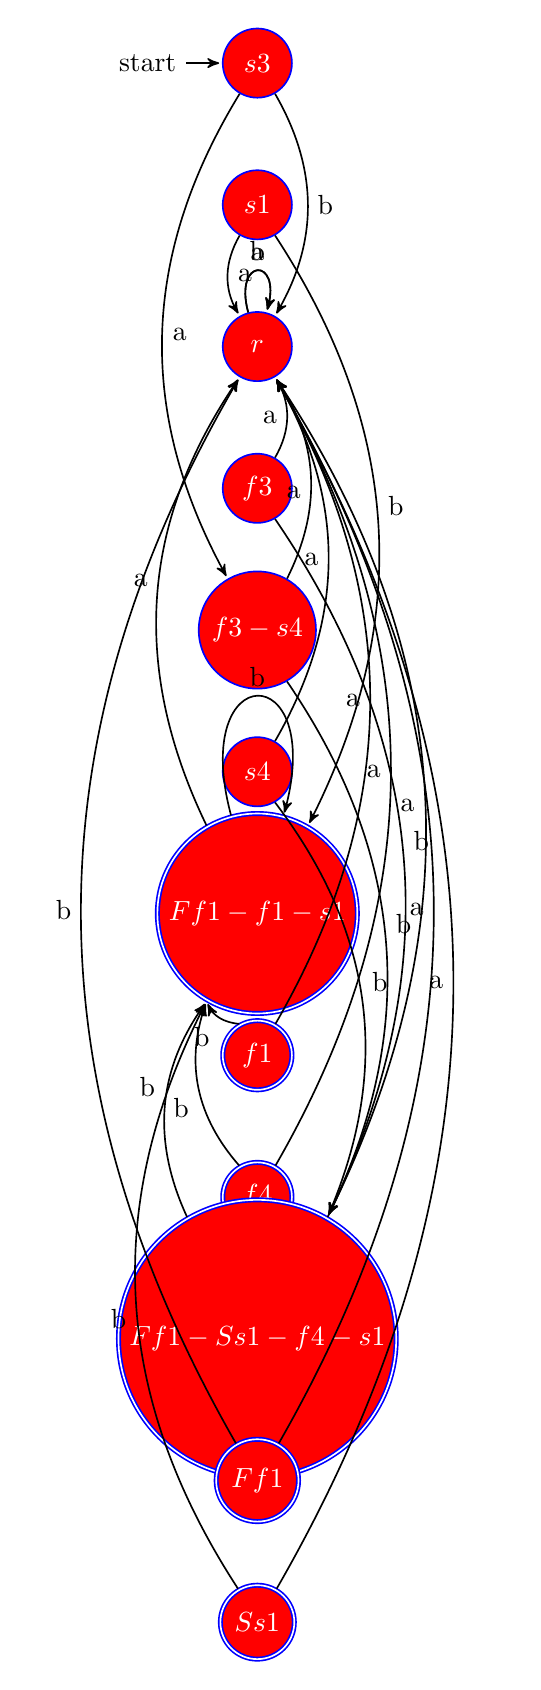
\begin{tikzpicture}[->,>=stealth',shorten >=1pt,auto,node distance=1.8cm,semithick]
   \tikzstyle{every state}=[fill=red,draw=blue,text=white]
   \node[state,initial]   (s3)        {$s3$};
   \node[state]   (s1)  [below of=s3]  {$s1$};
   \node[state]   (r)  [below of=s1]  {$r$};
   \node[state]   (f3)  [below of=r]  {$f3$};
   \node[state]   (f3-s4)  [below of=f3]  {$f3-s4$};
   \node[state]   (s4)  [below of=f3-s4]  {$s4$};
   \node[state,accepting]   (Ff1-f1-s1)  [below of=s4]  {$Ff1-f1-s1$};
   \node[state,accepting]   (f1)  [below of=Ff1-f1-s1]  {$f1$};
   \node[state,accepting]   (f4)  [below of=f1]  {$f4$};
   \node[state,accepting]   (Ff1-Ss1-f4-s1)  [below of=f4]  {$Ff1-Ss1-f4-s1$};
   \node[state,accepting]   (Ff1)  [below of=Ff1-Ss1-f4-s1]  {$Ff1$};
   \node[state,accepting]   (Ss1)  [below of=Ff1]  {$Ss1$};

   \path  
     (Ff1-f1-s1)  edge  [bend left]    node {a}  (r)
     (Ff1-f1-s1)  edge  [loop above]  node {b}  (Ff1-f1-s1)
     (s1)  edge  [bend right]    node {a}  (r)
     (s1)  edge  [bend left]    node {b}  (Ff1-f1-s1)
     (f1)  edge  [bend right]    node {a}  (r)
     (f1)  edge  [bend left]    node {b}  (Ff1-f1-s1)
     (f4)  edge  [bend right]    node {a}  (r)
     (f4)  edge  [bend left]    node {b}  (Ff1-f1-s1)
     (s3)  edge  [bend right]    node {a}  (f3-s4)
     (s3)  edge  [bend left]    node {b}  (r)
     (Ff1-Ss1-f4-s1)  edge  [bend right]    node {a}  (r)
     (Ff1-Ss1-f4-s1)  edge  [bend left]    node {b}  (Ff1-f1-s1)
     (r)  edge  [loop above]  node {a}  (r)
     (r)  edge  [loop above]  node {b}  (r)
     (Ff1)  edge  [bend right]    node {a}  (r)
     (Ff1)  edge  [bend left]    node {b}  (r)
     (f3)  edge  [bend right]    node {a}  (r)
     (f3)  edge  [bend left]    node {b}  (Ff1-Ss1-f4-s1)
     (Ss1)  edge  [bend right]    node {a}  (r)
     (Ss1)  edge  [bend left]    node {b}  (Ff1-f1-s1)
     (f3-s4)  edge  [bend right]    node {a}  (r)
     (f3-s4)  edge  [bend left]    node {b}  (Ff1-Ss1-f4-s1)
     (s4)  edge  [bend right]    node {a}  (r)
     (s4)  edge  [bend left]    node {b}  (Ff1-Ss1-f4-s1);
\end{tikzpicture}
\end{document}